\documentclass{article}


% Preamble
\usepackage{tikz}
\usetikzlibrary{calc} % for coordinate arithmetic

% Decorative box macro for D&D character sheets
% Usage: \dndbox{x}{y}{width}{height}
% where (x,y) is the lower-left corner

\newcommand{\dndbox}[4]{%
  % Parameters: #1 = x, #2 = y, #3 = width, #4 = height
  \pgfmathsetmacro{\cornersize}{0.15} % Size of corner decorations
  \pgfmathsetmacro{\inset}{0.05} % Inset for inner lines
  
  % Define coordinates
  \coordinate (ll) at (#1, #2);
  \coordinate (lr) at (#1 + #3, #2);
  \coordinate (ul) at (#1, #2 + #4);
  \coordinate (ur) at (#1 + #3, #2 + #4);
  
  % Main outer frame (heavy lines)
  \draw[line width=1.5pt] 
    ($(ll) + (\cornersize, 0)$) -- ($(lr) + (-\cornersize, 0)$)
    ($(lr) + (0, \cornersize)$) -- ($(ur) + (0, -\cornersize)$)
    ($(ur) + (-\cornersize, 0)$) -- ($(ul) + (\cornersize, 0)$)
    ($(ul) + (0, -\cornersize)$) -- ($(ll) + (0, \cornersize)$);
  
  % Corner decorations (ornate corners)
  % Lower-left corner
  \draw[line width=1.5pt] 
    ($(ll) + (\cornersize, 0)$) arc (0:90:\cornersize)
    ($(ll) + (0, \cornersize)$) -- ($(ll) + (0, \cornersize/2)$)
    ($(ll) + (\cornersize, 0)$) -- ($(ll) + (\cornersize/2, 0)$);
  \draw[line width=0.8pt] 
    ($(ll) + (\cornersize*0.7, \cornersize*0.3)$) arc (0:90:\cornersize*0.3);
    
  % Lower-right corner
  \draw[line width=1.5pt] 
    ($(lr) + (-\cornersize, 0)$) arc (180:90:\cornersize)
    ($(lr) + (0, \cornersize)$) -- ($(lr) + (0, \cornersize/2)$)
    ($(lr) + (-\cornersize, 0)$) -- ($(lr) + (-\cornersize/2, 0)$);
  \draw[line width=0.8pt] 
    ($(lr) + (-\cornersize*0.7, \cornersize*0.3)$) arc (180:90:\cornersize*0.3);
    
  % Upper-right corner
  \draw[line width=1.5pt] 
    ($(ur) + (-\cornersize, 0)$) arc (180:270:\cornersize)
    ($(ur) + (0, -\cornersize)$) -- ($(ur) + (0, -\cornersize/2)$)
    ($(ur) + (-\cornersize, 0)$) -- ($(ur) + (-\cornersize/2, 0)$);
  \draw[line width=0.8pt] 
    ($(ur) + (-\cornersize*0.7, -\cornersize*0.3)$) arc (180:270:\cornersize*0.3);
    
  % Upper-left corner
  \draw[line width=1.5pt] 
    ($(ul) + (\cornersize, 0)$) arc (0:-90:\cornersize)
    ($(ul) + (0, -\cornersize)$) -- ($(ul) + (0, -\cornersize/2)$)
    ($(ul) + (\cornersize, 0)$) -- ($(ul) + (\cornersize/2, 0)$);
  \draw[line width=0.8pt] 
    ($(ul) + (\cornersize*0.7, -\cornersize*0.3)$) arc (0:-90:\cornersize*0.3);
  
  % Inner frame lines (lighter)
  \draw[line width=0.5pt]
    ($(ll) + (\inset, \inset)$) rectangle ($(ur) + (-\inset, -\inset)$);
  
  % Double line effect on sides
  \draw[line width=0.3pt]
    ($(ll) + (\inset*2, \cornersize*1.5)$) -- ($(ul) + (\inset*2, -\cornersize*1.5)$)
    ($(lr) + (-\inset*2, \cornersize*1.5)$) -- ($(ur) + (-\inset*2, -\cornersize*1.5)$);
}

% Example usage:
% \begin{tikzpicture}
%   \dndbox{0}{0}{6}{4}
%   \node[text width=5.5cm, align=left] at (3, 2) {Content goes here};
% \end{tikzpicture}

\begin{document}

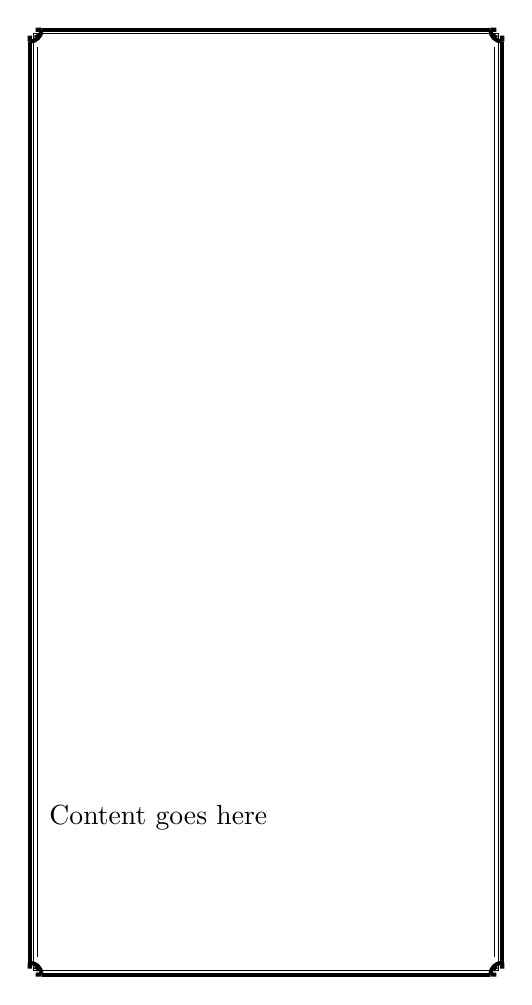
\begin{tikzpicture}
  \dndbox{0}{0}{6cm}{12cm}
  \node[text width=5.5cm, align=left] at (3, 2) {Content goes here};
\end{tikzpicture}

\end{document}


OK, let's start with a latex macro to create boxes with decorations, as are use for proficiencies, equipment, and so on.  The macro should be suitable to use inside a tikzpicture environment, using tikz, and it should take these parameters: the coordinates of the lower-left corner, and the width and height of the box.  Organize the parameters in whatever way makes the implementation simple.

Please be sure to reproduce these two aspects of the example: the mix of heavy and light rules, and the fancy corners.


Excellent!  As our next step, please define a utility {\LaTeX}
environment \begin{dndsection} for setting up a section.  It should take the same parameters as the \dndbox macro, and in addition it should take a title and a background color.   That environment should do the following:

  - Place a decorative box of the requested size at the requested location
  - Set the given background color inside the box
  - Place the title centered at the bottom, as in the examples
  - Set up a minipage environment for typesetting inside the box.

Leave a small margin between the minipage and the edges of the box, as shown in the example.

Note that the size of the box should be independent of the eventual height of the minipage.  Making things fit is the job of the user, not the environment.

Once you've done that, use your dndsection environment to define environments for each of the following sections:
attacks, magic, features, equipment, and proficiencies.

Finally, emit a sample page with all these sections, so I can test things.




\colorlet{stats}{blue!10!white}
\colorlet{proficiencies}{yellow!12!white}
\colorlet{attacks}{orange!25!white}
\colorlet{magic}{red!12!white}
\colorlet{mypurple}{red!40!blue}
\colorlet{feats}{magenta!16}
\colorlet{playername}{green!90!yellow!8!white}
\colorlet{teal}{blue!40!green}
\colorlet{equipment}{playername}
